\PassOptionsToPackage{table}{xcolor} % Fuer xcolor (option clash vermeiden)
\usepackage{xcolor} % Farben

%\usepackage[letterspace=200]{microtype} % Mikrokerning fuer sehr exakte Schriftarten
					% Einheit: 1/1000 eines em

\usepackage[left=3.00cm, right=3.00cm, top=3.00cm, bottom=3.00cm]{geometry} % Seitengeometrie

\usepackage[sfdefault]{noto} % Standardschrift aendern

\usepackage[T1]{fontenc} % Encoding
\usepackage[utf8]{inputenc}
\usepackage[ngerman]{babel} % Woerterbuch

\usepackage{sourcecodepro} % Standardschrift fuer Listings

\usepackage{listings} % Listings formatieren

\usepackage[german,algochapter]{algorithm2e} % Algorithmen
\SetAlFnt{\sffamily\small} %setzt den Font für die Algorithmen
\newcommand{\myAlgoFont}[1]{\small\textbf{\sffamily{#1}}}
\SetKwSty{myAlgoFont}
%Für algorithm2e Package die Caption setzen
\SetAlCapFnt{\sffamily\footnotesize}
\SetAlCapNameFnt{\sffamily\footnotesize}


\usepackage{csquotes}
\usepackage[justification=RaggedRight, singlelinecheck=false]{caption}
\usepackage{lstlinebgrd}

\usepackage{enumitem} % Aufzaehlungen mit eigenem Gliederungspunkt

\bibliographystyle{is-unsrt}

\usepackage[
    backend=biber,
    %style=is-unsrt,
    sortlocale=de_DE,
    natbib=true,
    url=false, 
    doi=true,
    eprint=false,
    backref=true %% In den Literaturangaben anzeigen, an welchen Stellen/Seiten das Zitat gesetzt ist
]{biblatex}
\addbibresource{main.bib} 
\usepackage{hyperref}

\usepackage{amsmath}

%%% In den Literaturangaben anzeigen, an welchen Stellen/Seiten das Zitat gesetzt ist
\DefineBibliographyStrings{german}{%
  backrefpage = {Seite},% originally "cited on page"
  backrefpages = {Seiten},% originally "cited on pages"
}


\usepackage{multicol}
\setlength{\columnsep}{1cm}

%\usepackage[singlespacing]{setspace} % Zeilenabstand Fliesstext normal
\usepackage[onehalfspacing]{setspace} % Zeilenabstand Fliesstext gedehnt
%\usepackage[doublespacing]{setspace} % Zeilenabstand Fliesstext doppelt gedehnt

\usepackage{adjustbox}

\usepackage{tabu} 
\usepackage{longtable}
\usepackage[table]{xcolor}
%\usepackage{float}
\usepackage{rotating}


%% Grafiken anzeigen:
\usepackage{graphicx}
%\usepackage[demo]{graphicx} % Grafiken im Schnellmodus (nur Boxen)

%% Beschriftungen neben Grafiken
\usepackage{floatrow}

%% Bilder als vorläufig markieren
\usepackage{overpic}
\newcommand{\draftImage}[2]{
	\begin{overpic}[#1]{#2}
		  \put(0,0){\includegraphics[#1]{#2}}
		    \put(15,5){\fontsize{30}{35}{\textbf{\begin{rotate}{45}VORLÄUFIG\end{rotate}}}}
	\end{overpic}
	}


\usepackage{nameref}


%% Randhinweise auch mit Grafiken
% Umgebung für Anmerkungen im Text
% (für den spacing-Befehl wird das setspace-Paket benötigt)
\usepackage{setspace}
% gelbe Hintergrundfarbe für Marginalie
\definecolor{sidebox_bg}{rgb}{1,1,0.4}
\newcommand{\sidenoteSingle}[1]{
        \hspace{0pt}%
        \marginpar{%
                \begin{spacing}{0.8}% Für geringeren Zeilenabstand
                        \fcolorbox{black}{sidebox_bg}{%
                                \parbox{.5\marginparwidth} {
                                        %\raggedright\sffamily\footnotesize{#1}%
                                        \sffamily\footnotesize{
						\begin{center}
							#1
							\vspace{2\baselineskip}
                                                \end{center}
					}%
                                }
                        }%
                \end{spacing}
        }
}

\newenvironment{androidversion}[1]%
    {\hspace{0pt}%    
     \marginpar{%
                %\vspace{1.8cm}
        \begin{spacing}{0.8}%
           %\fcolorbox{black}{sidebox_bg}{%
                \parbox{.5\marginparwidth}
                {
                        %\vspace{1.8cm}
                  \center
                        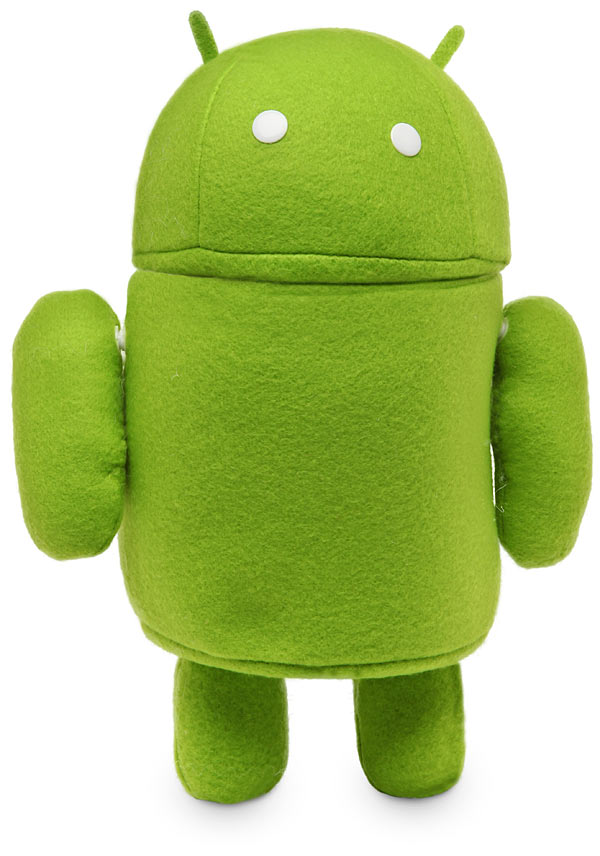
\includegraphics[width=.5\marginparwidth]{android_plush_robot.jpg}\
              \raggedright\sffamily
              \footnotesize{
                                                                \begin{center}
                                                                        Android~#1
                                                                        \vspace{2\baselineskip}
                                                                \end{center}                                   
                }%
                }          
        \end{spacing}
     }%
     }%
    {}%




%% Farbdefinitionen %%
\definecolor{color_c_comments}{rgb}{0.2, 0.7, 0.2}
\definecolor{color_c_keywords}{rgb}{1.0, 0.4, 0}
\definecolor{color_c_strings}{RGB}{180,116,19}
\definecolor{color_c_numbers}{rgb}{0.3, 0.3, 0.3}
\definecolor{color_bash_numbers}{rgb}{0.3, 0.3, 0.3}
\definecolor{color_lst_orange_light}{RGB}{255,250,241}


\definecolor{color_lst_gray_light}{RGB}{249,249,249}
\definecolor{color_keywords_background}{RGB}{255,238,205}
\definecolor{color_keywords_border}{rgb}{0.3, 0.3, 0.3}

\definecolor{tableHeader}{RGB}{255,238,205}
\definecolor{tableLineOne}{RGB}{245, 245, 245}
\definecolor{tableLineTwo}{RGB}{224, 224, 224}

\usepackage{tcolorbox} % Farbboxen
\newtcolorbox{importantbox}[1]{colback=red!5!white,
colframe=red!75!black,fonttitle=\bfseries,
title=#1}

%\newcommand{\keyword}[1]{\colorbox{color_keywords_background}{\texttt{#1}}} % Keywords ohne Box
\newcommand{\keyword}[1]{\adjustbox{margin=5pt 3pt, bgcolor=color_keywords_background, cfbox=orange 0.5pt 0pt, padding=2pt}{\texttt{#1}}} % Keywords mit Box
\newcommand{\srckeyword}[1]{\adjustbox{margin=5pt 3pt, bgcolor=color_lst_gray_light, cfbox=gray 0.5pt 0pt, padding=2pt}{\texttt{#1}}} % margin zuvor = 5pt 2pt 5pt 6pt

% Listings fuer Shellkommandos
\newcommand{\lstinputbash}[2]{
	\lstinputlisting[language=bash, #2, rulecolor=\color{gray},
		linebackgroundcolor={\ifodd\value{lstnumber}\color{color_lst_gray_light}\fi}
	]{#1}
}

\newcommand{\ignore}[1]{}
\newcommand{\pageWidth}{16.5cm}
%\newcommand{\quotes}[1]{``#1''}
\newcommand{\quotes}[1]{\glqq#1\grqq}
\newcommand{\techquotes}[1]{``#1''}

%% Tabellenstil mit Farbe
\newcommand{\tableHeaderStyle}{
    \rowfont{\leavevmode\color{black}\bfseries}
    \rowcolor{orange}
} 
\taburowcolors[2] 2{tableLineOne .. tableLineTwo}
\tabulinesep = ^2mm_1mm
\everyrow{\tabucline[.4mm  white]{}}

%% Listingstil fuer Makefiles
\lstdefinelanguage{Makefile}{
  sensitive=false, % keywords are not case-sensitive
  morecomment=[l]{\#}, % l is for line comment
  morestring=[b]" % defines that strings are enclosed in double quotes,
}

% Makefile aus einer Datei einbinden
\newcommand{\makefileinputlisting}[2]{
	\lstinputlisting[language=Makefile, #2, rulecolor=\color{gray},linebackgroundcolor={\ifodd\value{lstnumber}\color{color_lst_gray_light}\fi}]{#1}
}

\DeclareGraphicsExtensions{.png} % Grafikangabe

%% Einstellungen fuer Listings
\renewcommand\lstlistingname{Listing}
\renewcommand\lstlistlistingname{Programmcode-Verzeichnis}
\captionsetup{justification=RaggedRight,font={sf},labelsep=endash,labelfont=bf}

\lstset{
	basicstyle          =    \fontsize{9}{10}\ttfamily,
	commentstyle        =    \color{color_c_comments},
	frame               =    single,
	numbers             =    left,
	numbersep           =    5pt,
	numberstyle         =    \tiny\color{color_c_numbers},
	keywordstyle        =    \color{color_c_keywords},
	showspaces          =    false,
	showstringspaces    =    false,
	stringstyle         =    \color{color_c_strings},
	tabsize             =    2,
	breaklines          =    true,
	captionpos          =    b,
	belowskip           =    1em,
	abovecaptionskip    =    1em,
	aboveskip           =    3em,
	rulecolor           =    \color{orange},
	language            =    C,
	linebackgroundcolor =    {\ifodd\value{lstnumber}\color{color_lst_orange_light}\fi}
}

%% Nur zur Demo, kann in einer realen Ausarbeitung weg:
\usepackage{blindtext}


%% Makro zur Zeichnung von Gitternetzen
\newcount \myheight
\newcommand{\platz}[1]{
	\myheight=#1
	\advance \myheight by -1
	\multiply \myheight by 5
	\setlength{\unitlength}{1mm}
	\definecolor{grau}{gray}{0.8}
	\begin{picture}(175, \myheight)
		\color{grau}
		\thinlines
		\multiput(0,0)(5,0){36}{\line(0,1){\myheight}}
		\multiput(0,0)(0,5){#1}{\line(1,0){175}}
	\end{picture}
	}

